\section*{A brief description of the CRISPR circuit using SBOL 2.0 data model}
We first give a brief description of the CRISPR-based repression module. We use bold font in the following text and figure captions to mark available data model in SBOL 2.0. Detailed description of properties of the data model is available in the~\href{http://sbolstandard.org/downloads/specification-data-model-2-0/}{Specification
  (Data Model 2.0)}.

First, consider the CRISPR-based Repression Template \sbol{ModuleDefinition} shown in the center of Figure~\ref{fig:fig-CRPb}. It provides a generic description of CRISPR-based repression behavior. Namely, it includes generic \emph{Cas9}, \emph{guide RNA} (gRNA), and \emph{target} DNA \sbol{FunctionalComponent} instances. It also includes a \emph{genetic production} \sbol{Interaction} that expresses a generic target gene product.  Finally, it includes a \emph{non-covalent binding} \sbol{Interaction} that forms the Cas9/gRNA complex (shown as dashed arrows), which in turn participates in an \emph{inhibition} \sbol{Interaction} to repress the target gene product production (shown with a tee-headed arrow). The CRISPR-based Repression Template is then instantiated to test a particular CRISPR-based repression device, CRPb, by the outer CRPb Characterization Circuit \sbol{ModuleDefinition}.  This outer characterization circuit includes gene \sbol{FunctionalComponents} to produce specific products (i.e., mKate, Gal4VP16, cas9m\_BFP, gRNA\_b, and EYFP), as well as \sbol{FunctionalComponents} for the products themselves.  Next, it includes \emph{genetic production} \sbol{Interactions} connecting the genes to their products, and it has a \emph{stimulation} \sbol{Interaction} that indicates that Gal4VP16 stimulates production of EYFP.  Finally, it uses \sbol{MapsTo} objects (shown as dashed lines) to connect the generic \sbol{FunctionalComponents} in the template to the specific objects in the outer \sbol{ModuleDefinition}.  For example, the outer module indicates that the target protein is EYFP, while the cas9\_gRNA complex is cas9m\_BFP\_gRNA\_b.

\begin{figure}[tbph]
\begin{center}
  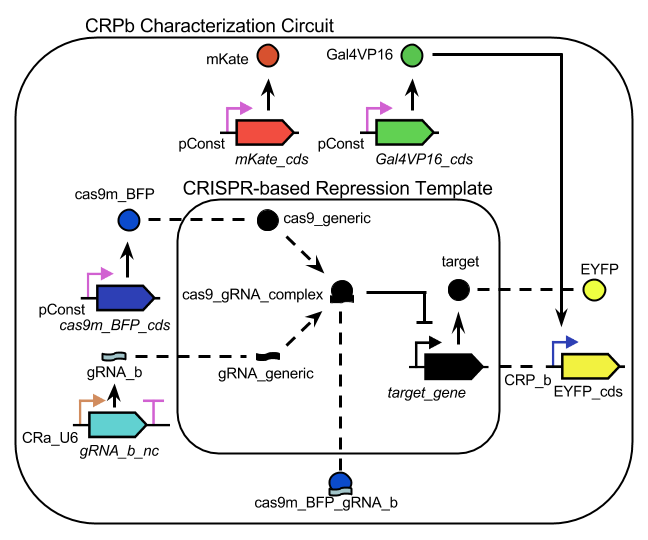
\includegraphics[width=0.95\textwidth]{figures/crispr_repression2} 
\end{center}
\caption{\label{fig:fig-CRPb} Illustration of a hierarchical CRISPR-based repression module represented in SBOL 2.0 (adapted from Figure~1a in \cite{kiani2014crispr}). The CRISPR-based Repression Template \sbol{ModuleDefinition} describes a generic CRISPR repression circuit that combines a Cas9 protein with a gRNA to form a complex (represented by the dashed arrows) that represses a target gene (represented by the arrow with the tee arrowhead).  These relationships between these \sbol{FunctionalComponents} (instances of \sbol{ComponentDefinitions}) are represented in SBOL 2.0 using \sbol{Interactions}.  This \sbol{Module} is instantiated in the outer CRPb Characterization Circuit \sbol{ModuleDefinition} in order to specify the precise (including \sbol{Sequences} when provided) \sbol{FunctionalComponents}  used for each generic \sbol{FunctionalComponent}. The undirected dashed lines going into the template \sbol{Module} represent \sbol{MapsTo} objects that specify how specific \sbol{FunctionalComponents} replace the generic ones.}
\end{figure}

\section*{Modeling CRISPR repression using {\tt libSBOLj 2.0}}

\subsection*{Setting up the CRISPR repression model}
Now we are ready to create the CRISPR model to our project. When the ``crispr'' project was created, two template Java class files ``App.java'' and ``AppTest.java'' were automatically created as shown below. 
\begin{center}
  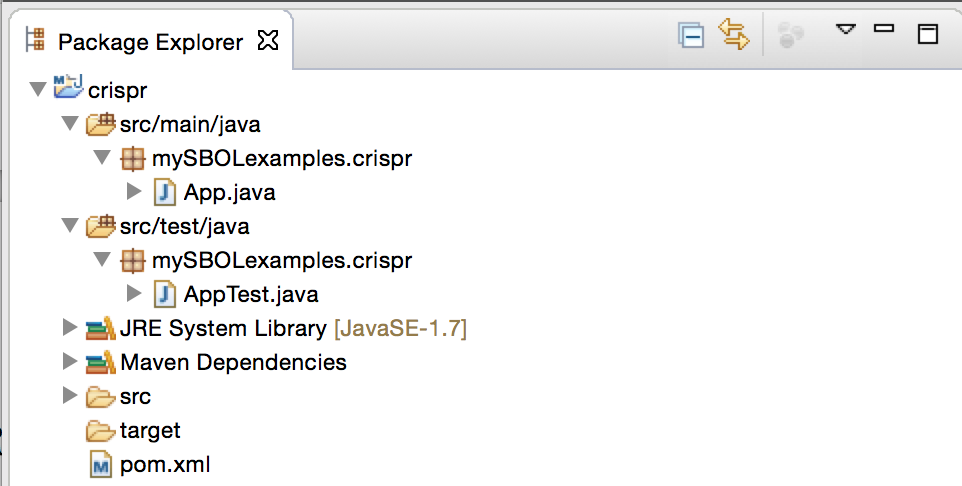
\includegraphics[width=0.8\textwidth]{figures/addCrisprModel1}
\end{center}

We can modify ``App.java'' to build the CRISPR model. First, remove all lines in ``App.java'' except the first line, which contains its package information. Then, rename ``App.java'' to ``RepressionModel.java''. You may now copy the import statements shown below to this file.

\begin{minipage}{0.95\textwidth} 
\begin{lstlisting}
import java.net.URISyntaxException;
import javax.xml.stream.FactoryConfigurationError;
import javax.xml.stream.XMLStreamException;
import org.sbolstandard.core2.AccessType;
import org.sbolstandard.core2.ComponentDefinition;
import org.sbolstandard.core2.DirectionType;
import org.sbolstandard.core2.Interaction;
import org.sbolstandard.core2.Module;
import org.sbolstandard.core2.ModuleDefinition;
import org.sbolstandard.core2.RefinementType;
import org.sbolstandard.core2.RestrictionType;
import org.sbolstandard.core2.SBOLDocument;
import org.sbolstandard.core2.SBOLWriter;
import org.sbolstandard.core2.Sequence;
import org.sbolstandard.core2.SequenceOntology;
import org.sbolstandard.core2.SystemsBiologyOntology;
import uk.ac.ncl.intbio.core.io.CoreIoException;
\end{lstlisting}
\end{minipage}

\subsection*{Creating SBOL Document}
For simplicity, we put all of our code in the \lstinline+main+ method of the \lstinline+RepressionModel+ class. All SBOL data objects are organized within an \sbol{SBOLDocument} object. The \sbol{SBOLDocument} provides a rich set of methods to create, access, update, and delete each type of \sbol{TopLevel} object (i.e., \sbol{Collection}, \sbol{ModuleDefinition}, \sbol{ComponentDefinition}, \sbol{Sequence}, \sbol{Model}, or \sbol{GenericTopLevel}). Every SBOL object has a \emph{uniform resource identifier} (URI) and consists of properties that may refer to other objects, including non-\sbol{TopLevel} objects such as SequenceConstraint and Interaction objects. \texttt{libSBOLj 2.0} organizes the URI collections to enable efficient access, and validation of uniqueness. We first create an \sbol{SBOLDocument} object by calling its constructor as shown below.

\begin{minipage}{0.95\textwidth} 
\begin{lstlisting}
public class RepressionModel {
	public static void main(String[] args) throws URISyntaxException {
		SBOLDocument doc = new SBOLDocument();
		doc.setDefaultURIprefix("http://sbols.org/CRISPR_Example/");
		doc.setComplete(true);
		doc.setCreateDefaults(true);
  }
}
\end{lstlisting}
\end{minipage}

The method \lstinline+setDefaultURIprefix+ sets the
default URI prefix to the string ``http://sbols.org/CRISPR\_Example/''. All data objects created following this statement carry this default URI prefix.  The \lstinline+doc.setComplete(true)+ statement sets the ``complete'' flag to \lstinline+true+ for the given \lstinline+doc+. It means that the URI for each data object in the current \lstinline+doc+ can be dereferenced to a valid object in this \sbol{SBOLDocuemnt} object. Otherwise, the library throws an exception. Finally, the \lstinline+doc.setCreateDefaults(true)+ statement
sets the ``createDefaults'' flag to \lstinline+true+ for the given
\lstinline+doc+.  It means that when an object that must
reference either a \lstinline+Component+ or \lstinline+FunctionalComponent+ object and cannot find the component, but it can find a \lstinline+ComponentDefinition+ object
with the same \lstinline+displayId+, it creates a default \lstinline+Component+ or \lstinline+FunctionalComponent+ object with this \lstinline+displayId+ and references it.

\subsection*{Adding CRISPR-based Repression Template module}
\subsubsection*{Creating \sbol{TopLevel} objects}
We first create the CRISPR-based Repression Template module shown in Figure~\ref{SBOL2}. In this template, we include definitions for generic \emph{Cas9}, \emph{guide RNA} (gRNA), and \emph{target} DNA \sbol{FunctionalComponent} instances. They are encoded as \sbol{ComponentDefinition} objects. Creation of the generic Cas9 (line 3) \sbol{ComponentDefinition} is done by passing its \emph{displayId} ``cas9\_generic'', \emph{version} specified by the \lstinline+version+ string, and \emph{type} to the \lstinline+createComponentDefinition+ method. Every \sbol{ComponentDefinition} must contain one or more types, each of which is specified by a URI. A type specifies the component's category of biochemical or physical entity (for example DNA, protein, or small molecule). The generic Cas9's type is \lstinline+PROTEIN+, which is defined as the BioPAX ontology term for protein (\url{http://www.biopax.org/release/biopax-level3.owl\#Protein}). Other \sbol{ComponentDefinition} objects shown below are created in the same way. A \sbol{ComponentDefinition} object can optionally have one or more roles, also in the form of URIs. The \lstinline+target_gene+ on line 6 below has a role of \lstinline+PROMOTER+, defined as the \emph{Sequence Ontology} (SO) term ``SO:0000167'' (\url{http://identifiers.org/so/SO:0000167}) in the library.  We then create the \sbol{ModuleDefinition} template by calling the \lstinline+createModuleDefinition+ method with the displayId ``CRISPR\_Template'' and \lstinline+version+. 

\vspace{\abovedisplayskip}
\begin{minipage}{0.95\textwidth} 
\begin{lstlisting}
String version = "1.0";
doc.createComponentDefinition(
         "cas9_generic", 
         version, 
         ComponentDefinition.PROTEIN
         );
doc.createComponentDefinition(
        "gRNA_generic",
        version, 
        ComponentDefinition.RNA
        );
doc.createComponentDefinition(
        "cas9_gRNA_complex",
        version, 
        ComponentDefinition.COMPLEX
        );
doc.createComponentDefinition(
        "target_gene",
        version, 
        ComponentDefinition.DNA
        ).addRole(SequenceOntology.PROMOTER);
doc.createComponentDefinition(
        "target",
        version, 
        ComponentDefinition.PROTEIN);
ModuleDefinition  CRISPR_Template = doc.createModuleDefinition(
        "CRISPR_Template", 
        version
        );
\end{lstlisting}
\end{minipage}

Each of create methods in the library creates a \emph{compliant URI} with the following form:
\begin{center}
http://$\langle$prefix$\rangle$/$\langle$displayId$\rangle$/$\langle$version$\rangle$
\end{center}
using the default URI prefix and provided displayId and version. The \emph{$\langle$prefix$\rangle$} represents a URI for a namespace (for example, {\tt www.sbols.org/CRISPR\_Example}). The author of a \sbol{TopLevel} object, such as the \sbol{ModuleDefinition} object we just created, should use a URI prefix that either they own or an organization of which they are a member owns. When using compliant URIs, the owner of a prefix must ensure that the URI of any unique \sbol{TopLevel} object that contains the prefix also contains a unique  \emph{$\langle$displayId$\rangle$} or \emph{$\langle$version$\rangle$} portion. Multiple versions of an SBOL object can exist and would have compliant URIs that contain identical prefixes and displayIds, but each of these URIs would need to end with a unique version. Lastly, the compliant URI of a non-\sbol{TopLevel} object is identical to that of its parent object, except that its displayId is inserted between its parent's displayId and version. This form of compliant URIs is chosen to be easy to read, facilitate debugging, and support a more efficient means of looking up objects and checking URI uniqueness. 

\subsubsection*{Specifying Interactions}
We are now ready to specify the interactions in the repression template. The first one is the complex formation interaction for \lstinline+cas9_generic+ and \lstinline+gRNA_generic+. We first create an \sbol{Interaction} object \lstinline+Cas9Complex_Formation+ in \lstinline+CRISPR_Template+, with the displayId ``cas9\_complex\_formation'' and a non-covalent binding type (line 1 to 4). It is recommended that terms from the \emph{Systems Biology Ontology} (SBO)~\cite{Courtot2011} are used specify the types for interactions. Table 11 of the ~\href{http://sbolstandard.org/downloads/specification-data-model-2-0/}{Specification  (Data Model 2.0)} document provides a list of possible SBO terms for the types property and their corresponding URIs. 

Next, we add three participants to this interaction object. Each participant is modeled as a \sbol{Participation} object and it refers to the corresponding \sbol{FunctionalComponent} object. For example, the \lstinline+participant_cas9_generic+ \sbol{Participation} object refers to the \lstinline+cas9_generic+ \sbol{FunctionalComponent} object. Note that such an object does not exist yet, but since there exists a \lstinline+cas9_generic+ \sbol{ComponentDefinition} object, and the ``createDefaults'' of this \sbol{SBOLDocuemnt} is set to \lstinline+true+, a \sbol{FunctionalComponent} with the same displayId ``cas9\_generic'' is automatically created and it connects the reference from the \lstinline+participant_cas9_generic+ \sbol{Participation} to the \lstinline+cas9_generic+ \sbol{ComponentDefinition}. After this \sbol{Participation} object is created, we call the \lstinline+addRole+ method to assign the \lstinline+REACTANT+ role to it. The remaining two participants are created in a similar fashion.

\vspace{\abovedisplayskip}
\begin{minipage}{0.95\textwidth}%{\linewidth} 
\begin{lstlisting}
Interaction Cas9Complex_Formation = CRISPR_Template.createInteraction(
        "cas9_complex_formation", 
        SystemsBiologyOntology.NON_COVALENT_BINDING
        );
Cas9Complex_Formation.createParticipation(
        "participant_cas9_generic", 
        "cas9_generic").addRole(SystemsBiologyOntology.REACTANT);
Cas9Complex_Formation.createParticipation(
        "participant_gRNA_generic", 
        "gRNA_generic").addRole(SystemsBiologyOntology.REACTANT);
Cas9Complex_Formation.createParticipation(
        "participant_cas9_gRNA_complex", 
        "cas9_gRNA_complex").addRole(SystemsBiologyOntology.PRODUCT);
\end{lstlisting}
\end{minipage}

The remaining two interactions, namely the genetic production of the target protein from the \lstinline+target_gene+ and the inhibition of the target protein by the \lstinline+cas9_gRNA_complex+, are specified using the same method calls.

\vspace{\abovedisplayskip}
\begin{minipage}{0.95\textwidth}%{\linewidth} 
\begin{lstlisting}
// Production of target from target gene
Interaction EYFP_production = CRISPR_Template.createInteraction(
        "target_production", 
        SystemsBiologyOntology.GENETIC_PRODUCTION
        );
EYFP_production.createParticipation(
        "participant_target_gene", 
        "target_gene").addRole(SystemsBiologyOntology.PROMOTER);
EYFP_production.createParticipation(
        "participant_target", 
        "target").addRole(SystemsBiologyOntology.PRODUCT);
	
// Inhibition of target by cas9m_BFP_gRNA 
Interaction target_generic_gene_inhibition = CRISPR_Template.createInteraction(
        "target_gene_inhibition", 
        SystemsBiologyOntology.INHIBITION
        );
target_generic_gene_inhibition.createParticipation(
        "participant_cas9_gRNA_complex", 
        "cas9_gRNA_complex").addRole(SystemsBiologyOntology.INHIBITOR);
target_generic_gene_inhibition.createParticipation(
        "participant_target_gene", 
        "target_gene").addRole(SystemsBiologyOntology.PROMOTER);
\end{lstlisting}
\end{minipage}

\subsection*{Creating CRPb Characterization Circuit}
So far, we have completed the repression template. In order to build the CRPb Characterization Circuit, we need to add precise (including \sbol{Sequences} when provided) \sbol{FunctionalComponents} used for each generic \sbol{FunctionalComponent} in the template. We first create \sbol{Sequence} objects for those provided in \cite{kiani2014crispr}\footnote{Unfortunately, as usual, not all sequences are provided in the paper.} as shown in the code below. For example, to create the sequence for the CRP\_b promoter, we call the \lstinline+createSequence+ method, as shown on line 57, with the displayId ``CRP\_b\_seq'', \lstinline+version+, the sequence specified by \lstinline+CRP_b_seq_elements+, and the IUPAC encoding for DNA, which is defined as a URI in the \sbol{Sequence} class, referencing \url{http://www.chem.qmul.ac.uk/iubmb/misc/naseq.html}.

\vspace{\abovedisplayskip}
\begin{minipage}{0.95\textwidth}%{\linewidth} 
\begin{lstlisting}[basicstyle=\tt\footnotesize]
// Create Sequence for CRa_U6 promoter
String CRa_U6_seq_elements = "GGTTTACCGAGCTCTTATTGGTTTTCAAACTTCATTGACTGTGCC" +
                "AAGGTCGGGCAGGAAGAGGGCCTATTTCCCATGATTCCTTCATAT" +
                "TTGCATATACGATACAAGGCTGTTAGAGAGATAATTAGAATTAAT" +
                "TTGACTGTAAACACAAAGATATTAGTACAAAATACGTGACGTAGA" +
                "AAGTAATAATTTCTTGGGTAGTTTGCAGTTTTAAAATTATGTTTT" +
                "AAAATGGACTATCATATGCTTACCGTAACTTGAAATATAGAACCG" +
                "ATCCTCCCATTGGTATATATTATAGAACCGATCCTCCCATTGGCT" +
                "TGTGGAAAGGACGAAACACCGTACCTCATCAGGAACATGTGTTTA" +
                "AGAGCTATGCTGGAAACAGCAGAAATAGCAAGTTTAAATAAGGCT" +
                "AGTCCGTTATCAACTTGAAAAAGTGGCACCGAGTCGGTGCTTTTT" +
                "TTGGTGCGTTTTTATGCTTGTAGTATTGTATAATGTTTTT";
doc.createSequence("CRa_U6_seq", version, CRa_U6_seq_elements, Sequence.IUPAC_DNA); 
		
// Create Sequence for gRNA_b coding sequence
String gRNA_b_elements = "AAGGTCGGGCAGGAAGAGGGCCTATTTCCCATGATTCCTTCATAT" +
                "TTGCATATACGATACAAGGCTGTTAGAGAGATAATTAGAATTAAT" +
                "TTGACTGTAAACACAAAGATATTAGTACAAAATACGTGACGTAGA" +
                "AAGTAATAATTTCTTGGGTAGTTTGCAGTTTTAAAATTATGTTTT" +
                "AAAATGGACTATCATATGCTTACCGTAACTTGAAAGTATTTCGAT" +
                "TTCTTGGCTTTATATATCTTGTGGAAAGGACGAAACACCGTACCT" +
                "CATCAGGAACATGTGTTTAAGAGCTATGCTGGAAACAGCAGAAAT" +
                "AGCAAGTTTAAATAAGGCTAGTCCGTTATCAACTTGAAAAAGTGG" +
                "CACCGAGTCGGTGCTTTTTTT";
doc.createSequence("gRNA_b_seq", version, gRNA_b_elements, Sequence.IUPAC_DNA);
		
// Create Sequence for mKate
String mKate_seq_elements = "TCTAAGGGCGAAGAGCTGATTAAGGAGAACATGCACATGAAGCTG" +
                "TACATGGAGGGCACCGTGAACAACCACCACTTCAAGTGCACATCC" +
                "GAGGGCGAAGGCAAGCCCTACGAGGGCACCCAGACCATGAGAATC" +
                "AAGGTGGTCGAGGGCGGCCCTCTCCCCTTCGCCTTCGACATCCTG" +
                "GCTACCAGCTTCATGTACGGCAGCAAAACCTTCATCAACCACACC" +
                "CAGGGCATCCCCGACTTCTTTAAGCAGTCCTTCCCTGAGGTAAGT" +
                "GGTCCTACCTCATCAGGAACATGTGTTTTAGAGCTAGAAATAGCA" +
                "AGTTAAAATAAGGCTAGTCCGTTATCAACTTGAAAAAGTGGCACC" +
                "GAGTCGGTGCTACTAACTCTCGAGTCTTCTTTTTTTTTTTCACAG" +
                "GGCTTCACATGGGAGAGAGTCACCACATACGAAGACGGGGGCGTG" +
                "CTGACCGCTACCCAGGACACCAGCCTCCAGGACGGCTGCCTCATC" +
                "TACAACGTCAAGATCAGAGGGGTGAACTTCCCATCCAACGGCCCT" +
                "GTGATGCAGAAGAAAACACTCGGCTGGGAGGCCTCCACCGAGATG" +
                "CTGTACCCCGCTGACGGCGGCCTGGAAGGCAGAAGCGACATGGCC" +
                "CTGAAGCTCGTGGGCGGGGGCCACCTGATCTGCAACTTGAAGACC" +
                "ACATACAGATCCAAGAAACCCGCTAAGAACCTCAAGATGCCCGGC" +
                "GTCTACTATGTGGACAGAAGACTGGAAAGAATCAAGGAGGCCGAC" +
                "AAAGAGACCTACGTCGAGCAGCACGAGGTGGCTGTGGCCAGATAC" +
                "TGCG";
doc.createSequence("mKate_seq", version, mKate_seq_elements, Sequence.IUPAC_DNA);

// Create Sequence for CRP_b promoter
String CRP_b_seq_elements =  "GCTCCGAATTTCTCGACAGATCTCATGTGATTACGCCAAGCTACG" +
                "GGCGGAGTACTGTCCTCCGAGCGGAGTACTGTCCTCCGAGCGGAG" +
                "TACTGTCCTCCGAGCGGAGTACTGTCCTCCGAGCGGAGTTCTGTC" +
                "CTCCGAGCGGAGACTCTAGATACCTCATCAGGAACATGTTGGAAT" +
                "TCTAGGCGTGTACGGTGGGAGGCCTATATAAGCAGAGCTCGTTTA" +
                "GTGAACCGTCAGATCGCCTCGAGTACCTCATCAGGAACATGTTGG" +
                "ATCCAATTCGACC";
doc.createSequence("CRP_b_seq", version, CRP_b_seq_elements, Sequence.IUPAC_DNA);
\end{lstlisting}
\end{minipage}

Next, we specify \sbol{ComponentDefinitions} for all \sbol{FunctionalComponents} in the CRPb Characterization Circuit. The code snippet below first creates a \sbol{ComponentDefinition} of DNA type for the \lstinline+CRP_b+ promoter (lines 1-7). Note that by using compliant URIs, the sequence can be looked up using its \emph{displayId}, i.e. \lstinline+CRP_b_seq+ that was added previously, and since no version is provided, it is referenced by its \emph{persistentIdentity} URI (line 7). It is simply its URI without the version when using compliant URIs. The purpose of a persistent identity is to allow an object to refer to the latest version of another object using this URI. The latest version of an object is determined using \emph{semantic versioning} conventions (c.f., \url{http://semver.org/}). Then, we create two \sbol{ComponentDefinition} objects, one for the EYFP \emph{coding sequence} (CDS), and one for the EYFP gene (lines 8-17). We use a \sbol{SequenceConstraint} object (lines 18-23) to indicate that the \lstinline+CRP_b+ promoter precedes the \lstinline+EYFP_cds+, because the sequence for the CDS has not been provided and thus cannot be given an exact \sbol{Range}. Note that since the ``createDefaults'' flag is set to \lstinline+true+, \sbol{FunctionalComponents} are automatically created for \lstinline+CRP_b+ and \lstinline+EYFP_cds+ \sbol{ComponentDefinition} objects, completing the reference from \lstinline+EYFP_gene_constraint+, via the \lstinline+CRP_b+ \sbol{FunctionalComponent}, to the \lstinline+CRP_b+ \sbol{ComponentDefinition}, and the reference from \lstinline+EYFP_gene_constraint+, via the \lstinline+EYFP_cds+ \sbol{FunctionalComponent}, to the \lstinline+EYFP_cds+ \sbol{ComponentDefinition}. 

Other \sbol{ComponentDefinition} objects can be created using the same set of method calls. As an exercise, the reader is encouraged to specify them according to Table~\ref{tbl:tbl-ComponentDef} and~\ref{tbl:tbl-SeqConstraint}. You can use the same \lstinline+version+ for all of the \sbol{ComponentDefinition} objects. Entries ``type'' column in the table are defined as constants in the \sbol{ComonentDefinition} class. Roles are SO terms defined as URI constants in the \sbol{SequenceOntology} class. URIs for these terms are described in Table 3 of the~\href{http://sbolstandard.org/downloads/specification-data-model-2-0/}{Specification  (Data Model 2.0)} document.

\vspace{\abovedisplayskip}
\begin{minipage}{0.95\textwidth}
\begin{lstlisting}
ComponentDefinition CRP_b = doc.createComponentDefinition(
        "CRP_b",
        version, 
        ComponentDefinition.DNA
        );
CRP_b.addRole(SequenceOntology.PROMOTER);
CRP_b.addSequence("CRP_b_seq");
doc.createComponentDefinition(
        "EYFP_cds", 
        version, 
        ComponentDefinition.DNA
        ).addRole(SequenceOntology.CDS);
ComponentDefinition EYFP_gene = doc.createComponentDefinition(
        "EYFP_gene", 
        version, 
        ComponentDefinition.DNA
        );
EYFP_gene.createSequenceConstraint(
        "EYFP_gene_constraint", 
        RestrictionType.PRECEDES, 
        "CRP_b", 
        "EYFP_cds"
        );
\end{lstlisting}
\end{minipage}

\begin{table}[tb]
\centering
\caption{\sbol{ComponentDefinition} objects}
\label{tbl:tbl-ComponentDef}
\begin{tabular}{c@{\hspace{1.5em}}c@{\hspace{1.5em}}cc@{\hspace{1.5em}}c}
\hline
component definition&
type&
role&
sequence&
sequence constraint\\
\hline
pConst&DNA&PROMOTER&n/a&n/a\\ %
cas9m\_BFP\_cds&DNA&CDS&n/a&n/a\\ %
cas9m\_BFP\_gene&DNA&PROMOTER&n/a&cas9m\_BFP\_gene\_constraint\\%
cas9m\_BFP&PROTEIN&n/a&n/a&n/a\\%
CRa\_U6&DNA&PROMOTER&CRa\_U6\_seq&n/a\\%
gRNA\_b\_nc&DNA&CDS&gRNA\_b\_seq&n/a\\%
gRNA\_b\_terminator&DNA&TERMINATOR&n/a&n/a\\%
gRNA\_b\_gene&DNA&PROMOTER&n/a&\begin{tabular}{@{}c@{}}\shortstack{\small{gRNA\_b\_gene\_constraint1} \\ \small{gRNA\_b\_gene\_constraint2}}\end{tabular}\\%
gRNA\_b&RNA&n/a&n/a&n/a\\%
cas9m\_BFP\_gRNA\_b&COMPLEX&n/a&n/a&n/a\\%
mKate\_cds&DNA&CDS&mKate\_seq&n/a\\%
mKate\_gene&DNA&PROMOTER&n/a&mKate\_gene\_constraint\\%
mKate&PROTEIN&n/a&n/a&n/a\\%
Gal4VP16\_cds&DNA&CDS&n/a&n/a\\%
Gal4VP16\_gene&DNA&PROMOTER&n/a&GAL4VP16\_gene\_constraint\\%
Gal4VP16&PROTEIN&n/a&n/a&n/a\\%
CRP\_b&DNA&PROMOTER&CRP\_b\_seq&n/a\\%
EYFP\_cds&DNA&CDS&n/a&n/a\\%
EYFP\_gene&DNA&PROMOTER&n/a&EYFP\_gene\_constraint\\%
EYFP&PROTEIN&n/a&n/a&n/a\\%
\hline
\end{tabular}%

\centering
\caption{\sbol{SequenceConstraint} objects}
\label{tbl:tbl-SeqConstraint}
\begin{tabular}{c@{\hspace{1.5em}}c@{\hspace{1.5em}}cc@{\hspace{1.5em}}c}
\hline
displayId&
restriction type&
subject&
object\\
\hline
cas9m\_BFP\_gene\_constraint&PRECEDES&pConst&cas9m\_BFP\_cds\\%
gRNA\_b\_gene\_constraint1&PRECEDES&CRa\_U6&gRNA\_b\_nc\\%
gRNA\_b\_gene\_constraint2&PRECEDES&gRNA\_b\_nc&gRNA\_b\_terminator\\%
mKate\_gene\_constraint&PRECEDES&pConst&mKate\_cds\\%
GAL4VP16\_gene\_constraint&PRECEDES&pConst&Gal4VP16\_cds\\%
EYFP\_gene\_constraint&PRECEDES&CRP\_b&EYFP\_cds\\%
\end{tabular}
\end{table}

We are now ready to create all remaining \sbol{FunctionalComponent} objects. We first create a \sbol{ModuleDefinition} object for the CRPb Characterization Circuit as shown below (lines 1-4). Then we create a \sbol{FunctionalComponent} \lstinline+EYFP+ that has a \sbol{PRIVATE} access type and refers to the \lstinline+EYFP+ \sbol{ComponentDefinition} object. The private access type means that this \sbol{FunctionalComponent} must not be referred to by remote \sbol{MapsTo} objects. Its direction property is \lstinline+NONE+, indicating that it serves neither input or output with regards to the \lstinline+CPRb_circuit+. Other \sbol{FunctionalComponent} objects, namely \lstinline+cas9m_BFP+, \lstinline+cas9m_BFP_gene+, \lstinline+gRNA_b+, \lstinline+gRNA_b_gene+, \lstinline+mKate+, \lstinline+mKate_gene+, \lstinline+Gal4VP16+, \lstinline+Gal4VP16_gene+, \lstinline+EYFP_gene+, and \lstinline+cas9m_BFP_gRNA_b+, can be created similarly with the same access type, version, and direction type. 

\vspace{\abovedisplayskip}
\begin{minipage}{0.95\textwidth}
\begin{lstlisting}
ModuleDefinition CRPb_circuit = doc.createModuleDefinition(
        "CRPb_characterization_circuit", 
        version
        );
CRPb_circuit.createFunctionalComponent(
        "EYFP", 
        AccessType.PRIVATE, 
        "EYFP", 
        version, 
        DirectionType.NONE);
\end{lstlisting}
\end{minipage}

Next, we need to specify all interactions for the CRPb Characterization Circuit. Following the same procedure for creating \sbol{Interactions} before, we can create those specified in Table~\ref{tbl:tbl-Interaction}. 

\begin{table}[tb]
\caption{\sbol{Interaction} objects}
\label{tbl:tbl-Interaction}
\centering
\begin{tabular}{c@{\hspace{1.5em}}c@{\hspace{1.5em}}c@{\hspace{1.5em}}c@{\hspace{1.5em}}}
\hline
interaction&
type&
participant&
role\\
\hline
\multirow{2}{*}{mKate\_production}&\multirow{2}{*}{GENETIC\_PRODUCTION}&mKate\_gene&PROMOTER\\
  &&mKate&PRODUCT\\ \hline %
\multirow{2}{*}{Gal4VP16\_production}&\multirow{2}{*}{GENETIC\_PRODUCTION}&Gal4VP16\_gene&PROMOTER\\
  &&Gal4VP16&PRODUCT\\ \hline %
\multirow{2}{*}{cas9m\_BFP\_production}&\multirow{2}{*}{GENETIC\_PRODUCTION}&cas9m\_BFP\_gene&PROMOTER\\
  &&cas9m\_BFP&PRODUCT\\ \hline %
\multirow{2}{*}{gRNA\_b\_production}&\multirow{2}{*}{GENETIC\_PRODUCTION}&gRNA\_b\_gene&PROMOTER\\
  &&gRNA\_b&PRODUCT\\ \hline %
\multirow{2}{*}{EYFP\_Activation}&\multirow{2}{*}{STIMULATION}&EYFP\_gene&PROMOTER\\
  &&Gal4VP16&STIMULATOR\\ \hline %
mKate\_deg&DEGRADATION&mKate&REACTANT\\ \hline%
GAL4VP16\_deg&DEGRADATION&GAL4VP16&REACTANT\\ \hline%
cas9m\_BFP\_deg&DEGRADATION&cas9m\_BFP&REACTANT\\ \hline%
gRNA\_b\_BFP\_deg&DEGRADATION&gRNA\_b\_BFP&REACTANT\\ \hline%
EYFP\_BFP\_deg&DEGRADATION&EYFP\_BFP&REACTANT\\ \hline%
cas9m\_BFP\_gRNA\_b\_BFP\_deg&DEGRADATION&cas9m\_BFP\_gRNA\_b\_BFP&REACTANT\\ \hline%
\end{tabular}
\end{table}

Now, the CRISPR-based Repression Template \sbol{Module} is instantiated and connected to the CRPb Characterization Circuit using \sbol{MapsTo} objects. The code below shows these mappings.
For example, a \sbol{MapsTo} object is used to indicate that the \texttt{target\_gene} in the template should be refined to be the \texttt{EYFP\_gene} specified in the CRPb circuit (lines 30-35).  

\vspace{\abovedisplayskip}
\begin{minipage}{0.95\textwidth}
\begin{lstlisting}
Module Template_Module = CRPb_circuit.createModule(
        "CRISPR_Template", 
        "CRISPR_Template", 
        version
        );
Template_Module.createMapsTo(
        "cas9m_BFP_map", 
        RefinementType.USELOCAL,
        "cas9m_BFP", 
        "cas9_generic"
        );
Template_Module.createMapsTo(
        "gRNA_b_map", 
        RefinementType.USELOCAL, 
        "gRNA_b", 
        "gRNA_generic"
        );
Template_Module.createMapsTo(
        "cas9m_BFP_gRNA_map", 
        RefinementType.USELOCAL, 
        "cas9m_BFP_gRNA_b", 
        "cas9_gRNA_complex"
        );
Template_Module.createMapsTo(
        "EYFP_map", 
        RefinementType.USELOCAL,
        "EYFP", 
        "target"
        );
Template_Module.createMapsTo(
        "EYFP_gene_map", 
        RefinementType.USELOCAL, 
        "EYFP_gene", 
        "target_gene"
        );
\end{lstlisting}
\end{minipage}

At this point, we have completed the CRISPR circuit model. One final step is to serialize the complete model to produce an RDF/XML output. This can be done by adding the code below.

\vspace{\abovedisplayskip}
\begin{minipage}{0.95\textwidth}
\begin{lstlisting}
try {
      SBOLWriter.write(doc, System.out);
}
catch (XMLStreamException | FactoryConfigurationError | CoreIoException e) {
      e.printStackTrace();
}
\end{lstlisting}
\end{minipage}

The complete repression model is described in the ``RepressionModel.java'' under the {\tt libSBOLj} examples directory. This example is self-contained in that you can run it to generate the RDF/XML output. Note that SBOL does not provide the specification of a mathematical model directly. It is possible, however, to generate a mathematical model using SBML~\cite{SBML} and the procedure described in~\cite{roehner2015generating}. Then, the SBOL document can reference this generated SBML model.

% The next section gives an introduction to some other methods provided by the API of {\tt libSBOLj}.
